\chapter{四足機械狗運動模擬}
將模型以剛體狀態導入CoppeliaSim模擬,在設定環境及轉軸後,利用Python進行控制。\
透過上述動作即可以找出作動角度範圍,用以推導運動方程及最大受力角度、使其運動軌跡和姿態符合設計需求,此步驟所解將用於有限元素分析。\
運用RemoteAPI將模型透過網際方式進行模擬,可用於遠端模擬並控制,可作為教學及演示用途。\\

\section{模型及環境設定}
\begin{figure}[hbt!]
\center
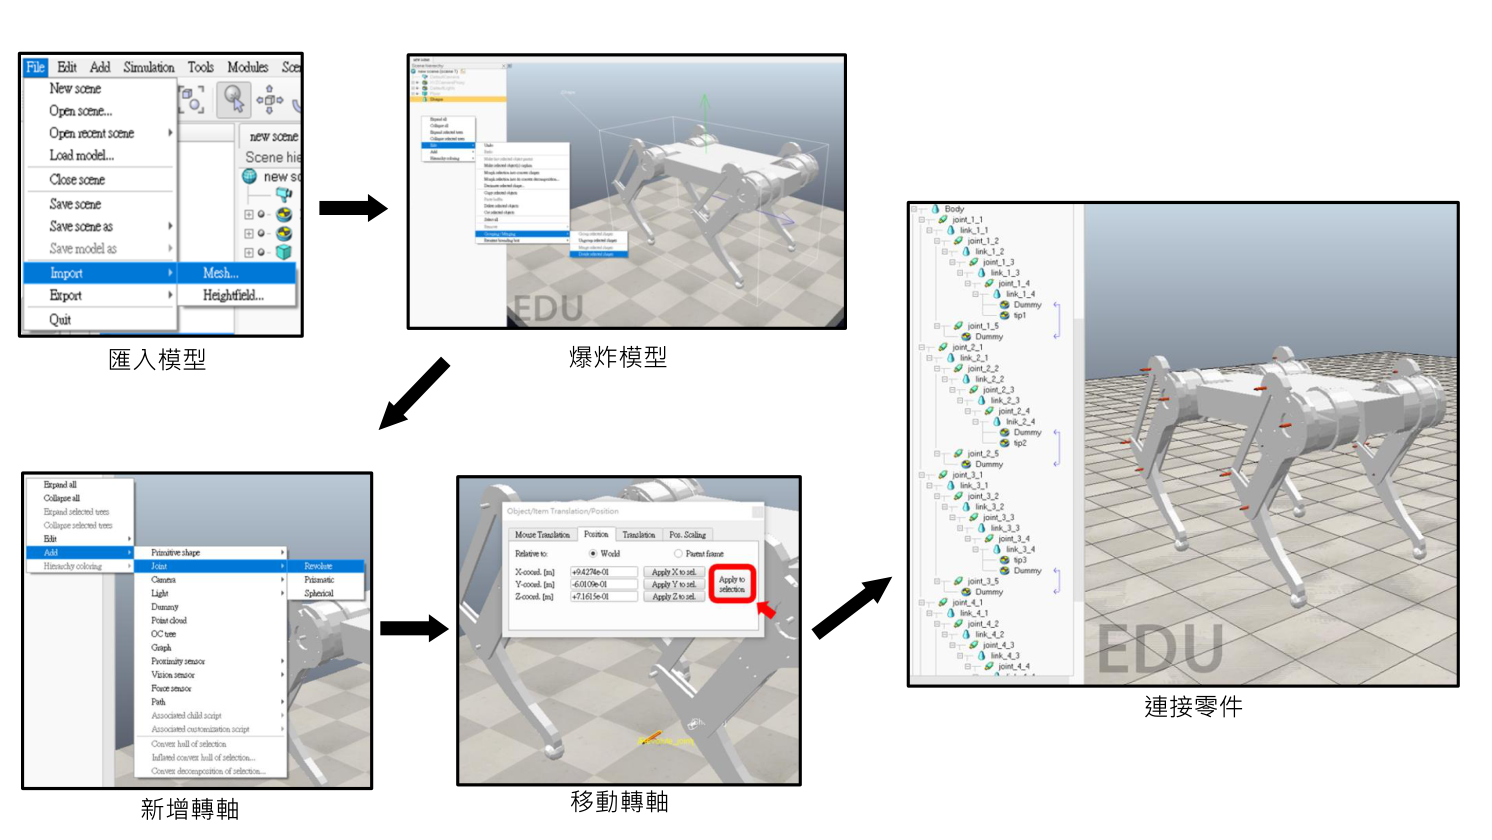
\includegraphics[width=10cm]{cop組裝步驟}
\caption{組裝步驟}\label{cop組裝步驟}
\end{figure}
\newpage
在此帶入所設計的四足機器狗,在每個旋轉關節插入轉軸並設定中修改零件的重量等參數,並設定環境參數給予物理引擎,令模型能夠以最為真實的情況進行模擬。\\

\begin{figure}[hbt!]
\center
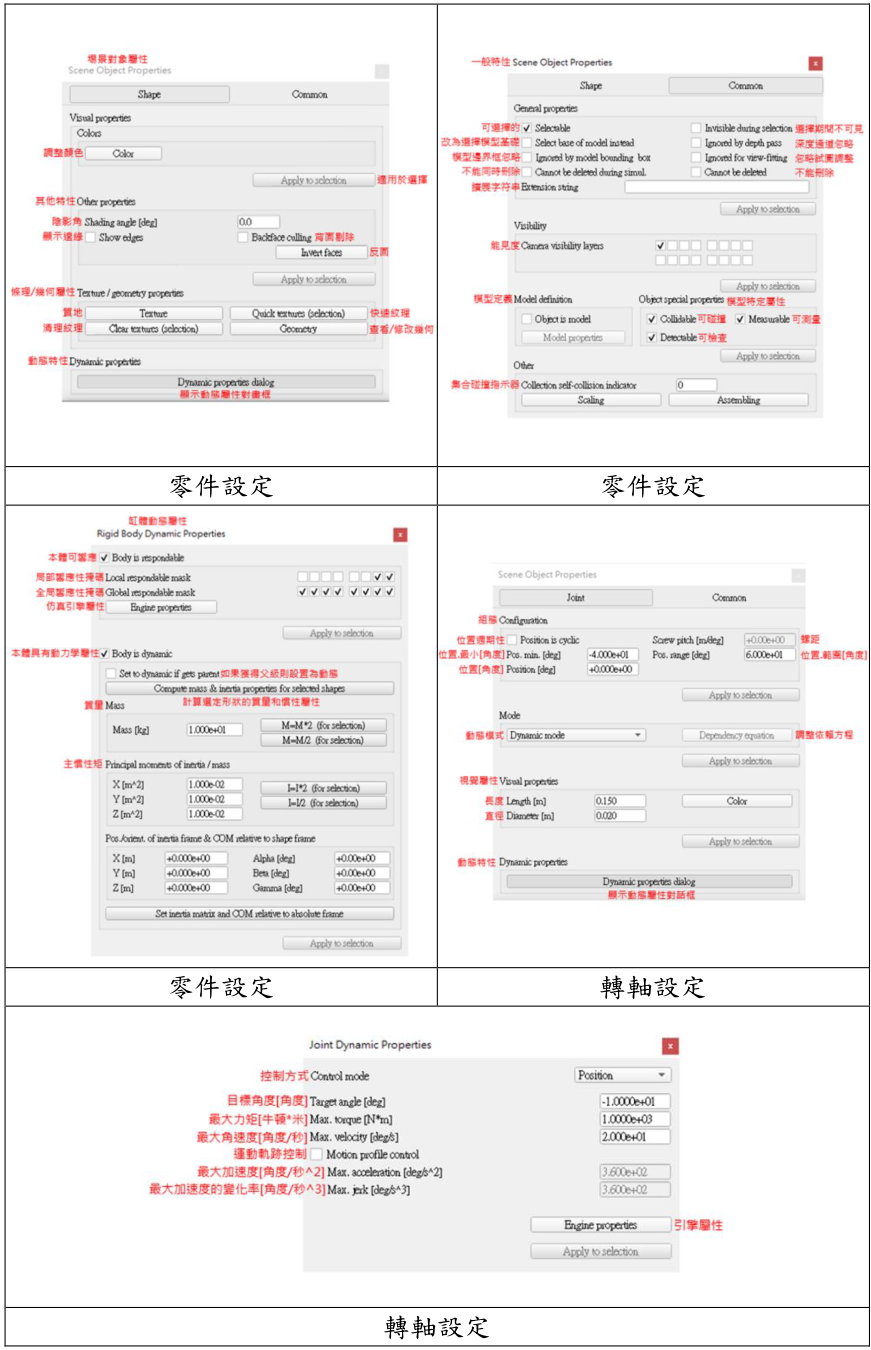
\includegraphics[width=13cm]{cop參數設定}
\caption{零件與轉軸參數設定}\label{cop參數設定}
\end{figure}
\newpage

\section{Python控制程式}
運動模擬主要以Python程式碼進行控制,優點有為可以遠端控制模擬、可依據運動學計算出角度控制末端點位置。\\

進行運動模擬控制時,我們在軟體控制中利用角度控制轉軸的所在位置,調用並定義需要控制的轉軸及函數,設置無限迴圈檢測目標按鍵為正確位置,再將先前定義的函數寫入迴圈,以上步驟完成後,即可控制每隻轉軸角度達成理想動作。\\


\label{模塊導入}
\begin{lstlisting}[caption=\Large 模塊導入]
from zmqRemoteApi import RemoteAPIClient 
import keyboard
import time

# 利用 zmqRemoteApi 中的 RemoteAPIClient 連結場景
client = RemoteAPIClient('localhost', 23000)
\end{lstlisting}

\begin{itemize}
\item API模塊 : 遠端通訊客戶端介面
\item keyboard模塊 : 檢測鍵盤輸入
\item time模塊 : 暫停當前程式一段時間
\item client : 導入遠端場景的地址和端口
\end{itemize}
以較為直覺且直觀的鍵盤進行控制,使用者可以依據自己的想法控制機器人做動\\

\label{啟動模擬}
\begin{lstlisting}[caption=\Large 啟動模擬]
print('Program started')
sim = client.getObject('sim')
sim.startSimulation()
print('Simulation started')
\end{lstlisting}
\begin{enumerate}
\item 輸出訊息表示程式開始運行
\item 與場景的連接
\item 啟動了場景中的模擬
\item 輸出一個訊息表示模擬已經開始運行。
\end{enumerate}

\label{轉軸設定}
\begin{lstlisting}[caption=\Large 轉軸設定]
#調用需要控制的轉軸
joint_1_1 = sim.getObject('/joint_1_1')
joint_1_2 = sim.getObject('/joint_1_2')
joint_2_1 = sim.getObject('/joint_2_1')
joint_2_2 = sim.getObject('/joint_2_2')
joint_3_1 = sim.getObject('/joint_3_1')
joint_3_2 = sim.getObject('/joint_3_2')
joint_4_1 = sim.getObject('/joint_4_1')
joint_4_2 = sim.getObject('/joint_4_2')
\end{lstlisting}  

調用需要控制的轉軸,代表場景中的不同關節,進一步用於操作和控制這些關節物件的行為。\\

\label{轉軸函數}
\begin{lstlisting}[caption=\Large 轉軸函數]
#定義控制轉軸函數 

def setJointPosition(target_angle1,target_angle2,
        target_angle3,target_angle4,target_angle5,
        target_angle6,target_angle7,target_angle8):

     sim.setJointTargetPosition(joint_1_1,
                target_angle1 * 3.14159 / 180)
     sim.setJointTargetPosition(joint_1_2,
                target_angle2 * 3.14159 / 180)
     sim.setJointTargetPosition(joint_2_1,
                target_angle3 * 3.14159 / 180)
     sim.setJointTargetPosition(joint_2_2,
                target_angle4 * 3.14159 / 180)
     sim.setJointTargetPosition(joint_3_1,
                target_angle5 * 3.14159 / 180)
     sim.setJointTargetPosition(joint_3_2,
                target_angle6 * 3.14159 / 180)
     sim.setJointTargetPosition(joint_4_1,
                target_angle7 * 3.14159 / 180)
     sim.setJointTargetPosition(joint_4_2,
                target_angle8 * 3.14159 / 180)
     
\end{lstlisting}
用於設定場景中關節的目標位置,目標角度設定為對應關節的目標位置,以便控制場景中的關節物件達到指定的角度位置。\\
\newpage


\label{鍵盤控制及角度設定}
\begin{lstlisting}[caption=\Large 鍵盤控制及角度設定]
#使用鍵盤移動模型
while True:
    if keyboard.is_pressed('q'):
        setJointPosition(20,20,-30,0,20,10,-30,0)
        time.sleep(0.5)
        setJointPosition(-30,0,20,10,-30,0,20,20)
        time.sleep(1)
    elif keyboard.is_pressed('w'):
        setJointPosition(-30,0,20,10,-30,0,20,5)
        time.sleep(0.5)
        setJointPosition(20,5,-30,10,20,10,-30,10)
        time.sleep(1)
    else:
        setJointPosition(-10,0,-10,0,-10,0,-10,0)
\end{lstlisting}
設定各關節目標位置並利用按鍵偵測確定選用哪條函式。\\

\section{運動模擬}
我們可以將四足機器人運動模式分為以下三種,分別為:\\

\begin{enumerate}
\item 爬行(Crawl):\
此動作較簡單且容易控制,作用在於機器人需緩慢移動或是穩定度需求高的情況下,由其中單腳前伸其餘進行關節旋轉,在小位移量的情況下實現行走功能。\
\item 小跑(Trot):\
此作用型態為FR+RL或FL+RR做動,進行移動時有著兩動兩不動的準則,在不動的部分做關節的旋轉運動,令四足機器人在快速移動下還能對身體保持平衡,在大位移量的情況下實現行走功能。\
\item 跳躍(Bound):\
由前兩足進行快速彈跳位移,使機器狗的關節進行快速調整以支撐身體姿態,分為FL+FR及RL+RR兩組,在躍障或其他特殊行為中使用。\
\end{enumerate}
\begin{figure}[hbt!]
\center
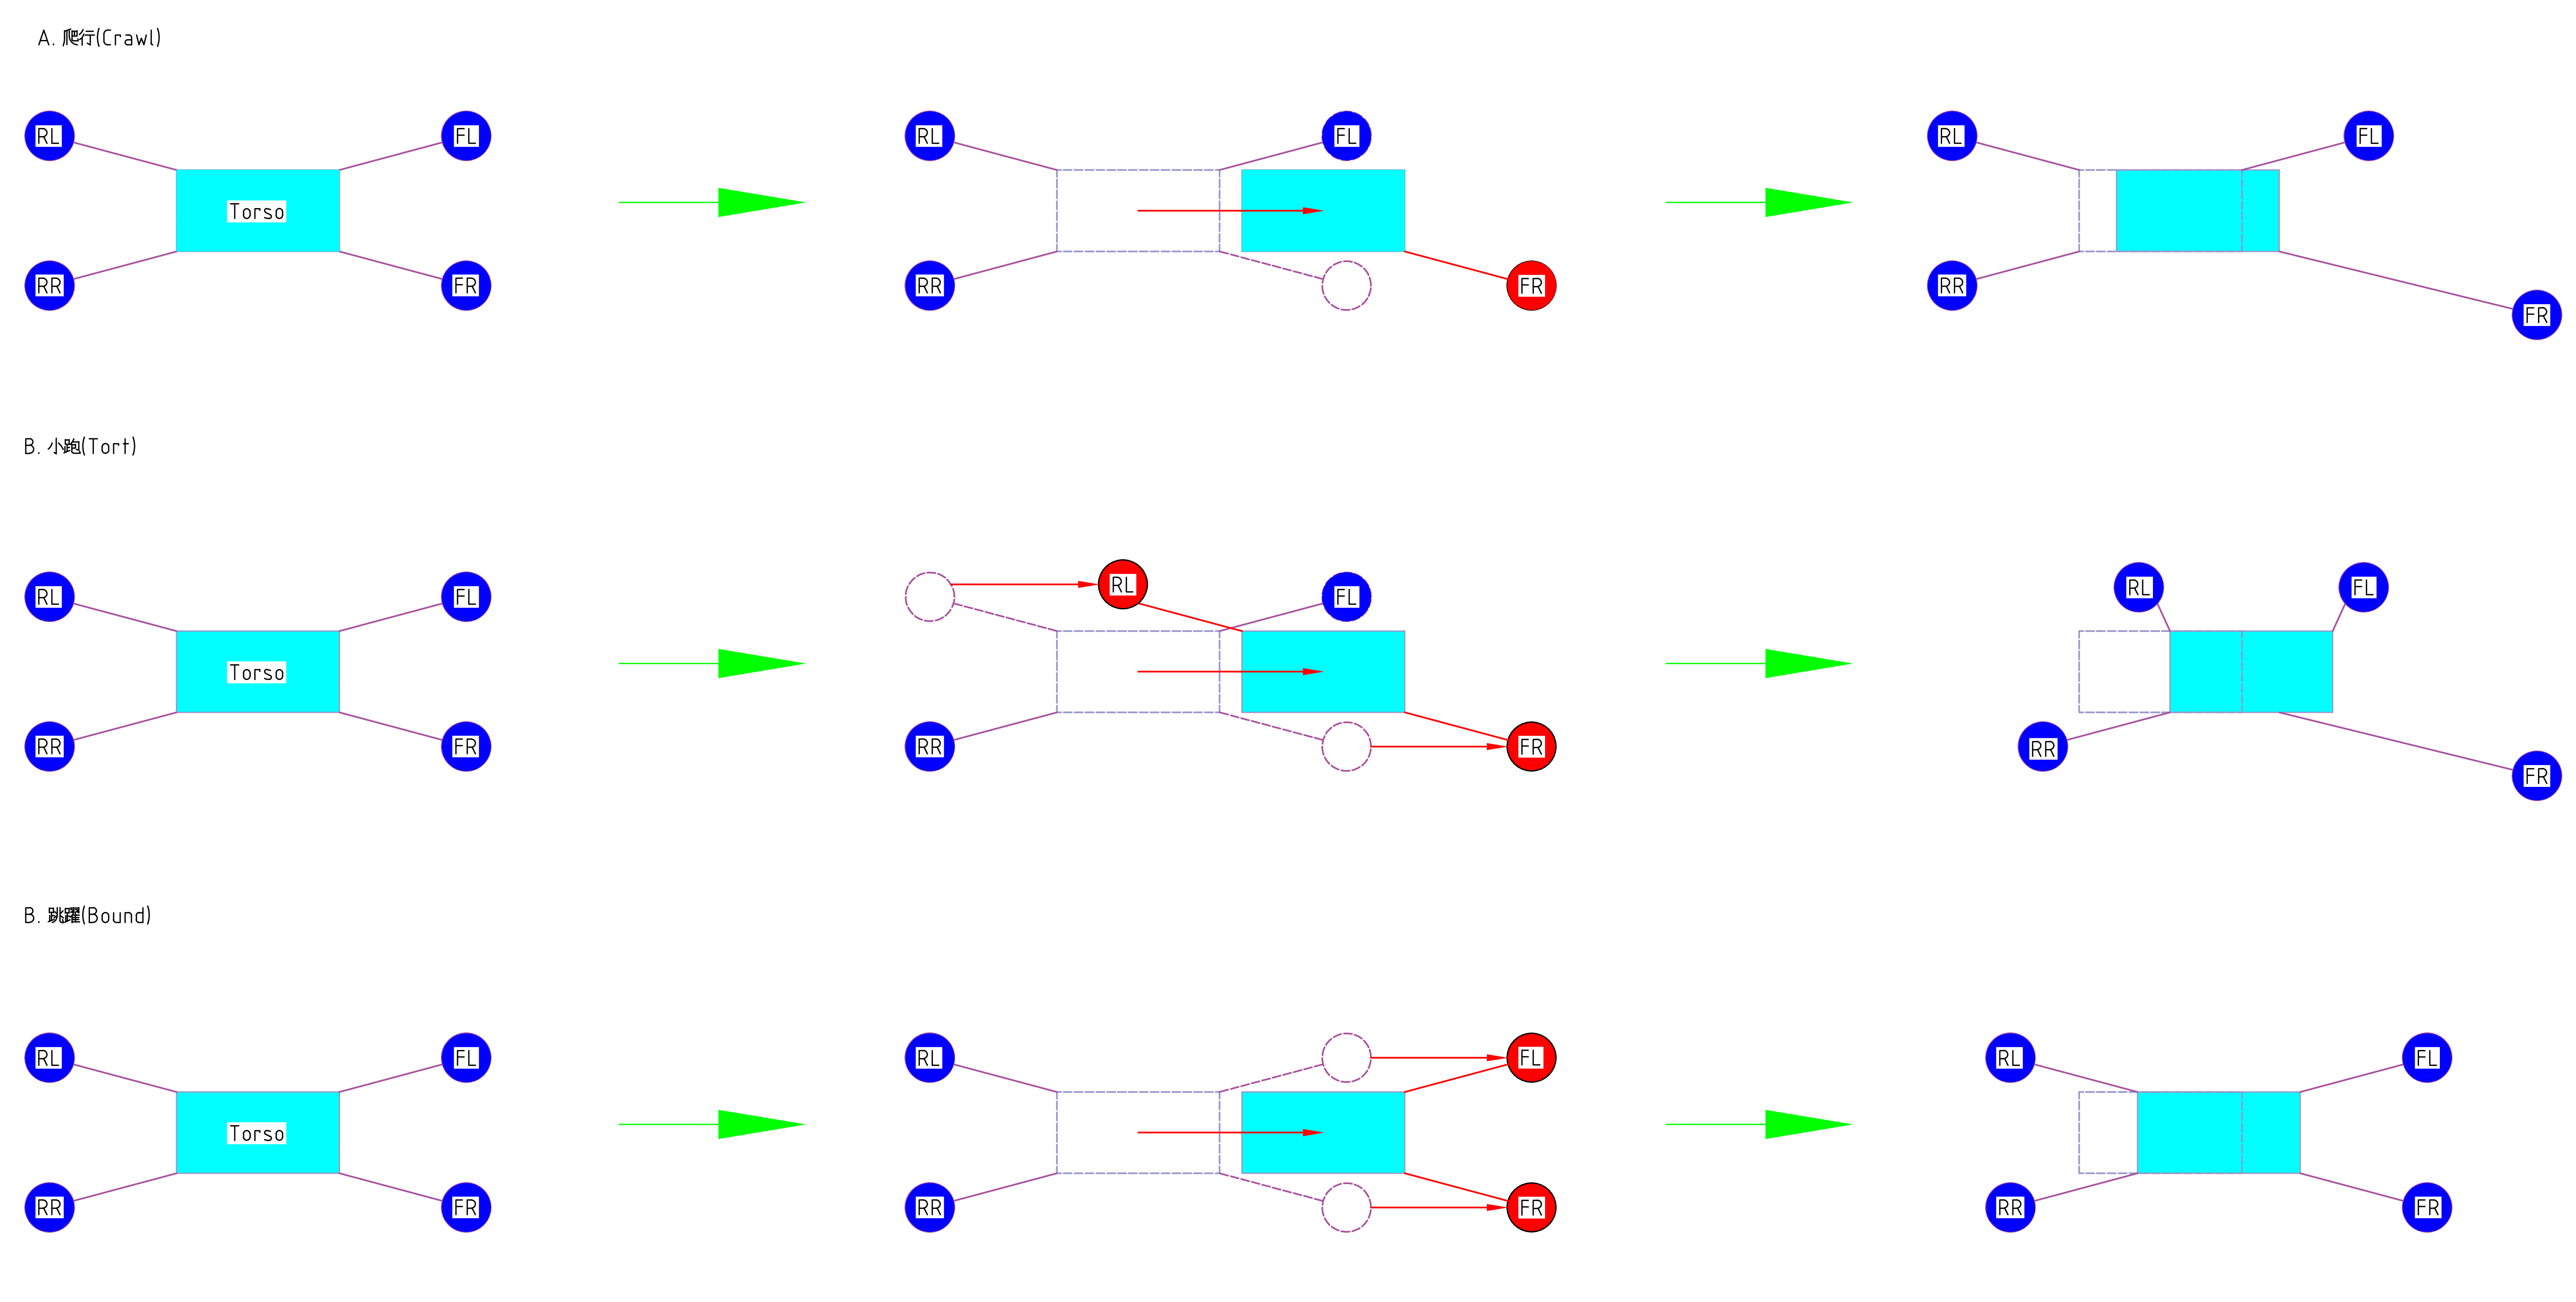
\includegraphics[width=13cm]{各式步態圖}
\caption{各式步態圖}\label{各式步態圖}
\end{figure}
\newpage


下列圖片為機器人在小跑時的模擬圖片:\
\begin{figure}[htbp]
  \begin{minipage}[t]{0.5\linewidth}
    \centering
    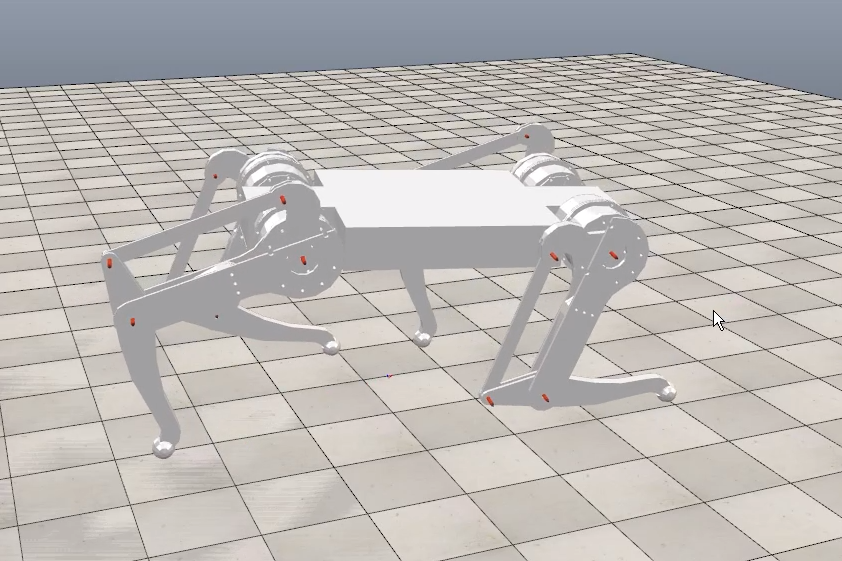
\includegraphics[height=6cm,width=6cm]{模擬動作-1}
    \caption{模擬動作-1}
    \label{模擬動作-1}
  \end{minipage}
  \hfill
  \begin{minipage}[t]{0.5\linewidth}
    \centering
    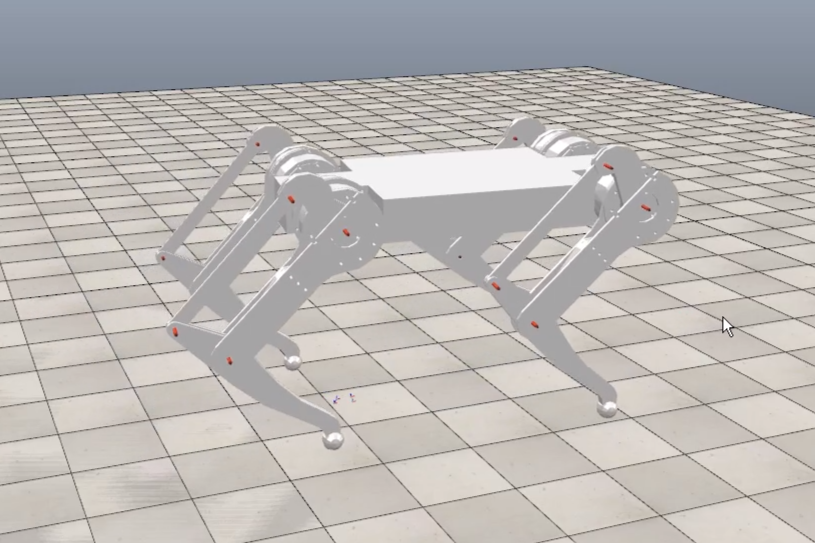
\includegraphics[height=6cm,width=6cm]{模擬動作-2}
    \caption{模擬動作-2}
    \label{模擬動作-2}
  \end{minipage}
\end{figure}

\begin{figure}[hbt!]
\begin{center}
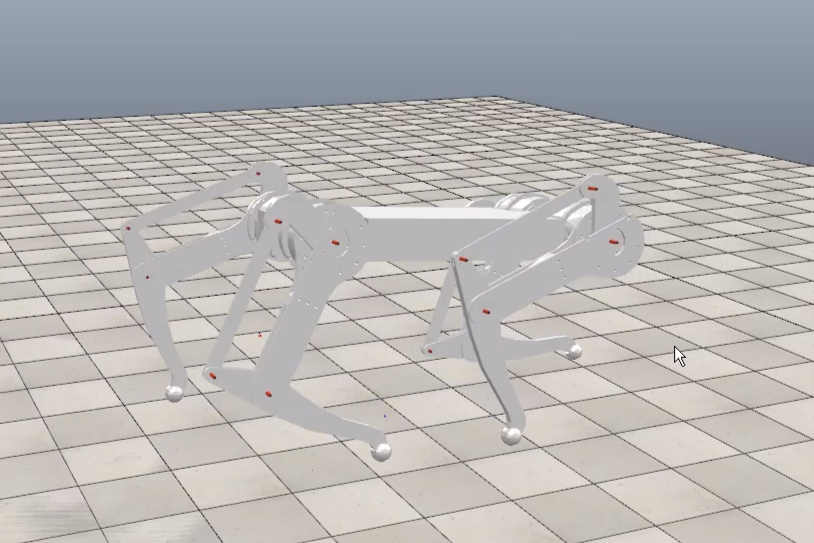
\includegraphics[height=6cm,width=6cm]{模擬動作-3}
\caption{\Large 模擬動作-3}\label{模擬動作-3}
\end{center}
\end{figure}
\newpage
